\documentclass[12pt]{article}
\usepackage[italian]{babel}
\usepackage{geometry}
\usepackage{amsmath}
\usepackage{graphicx}
\usepackage{amssymb}

\geometry{margin=2cm}

\title{Capitolo 1.1 - 1.2}
\author{Lorenzo Vaccarecci}
\date{26 Febbraio 2024}

\graphicspath{{./Immagini/}}
\newtheorem{definition}{Definizione}

\begin{document}
\maketitle
\section{Appunti vari}
Relazione \(P\) su \(I\times S\):
\begin{itemize}
    \setlength\itemsep{0em} 
    \item \(I\) insieme degli input
    \item \(S\) insieme delle soluzioni
\end{itemize}
\textbf{Problema \(\neq\) Algoritmo}
\\\\\textbf{Algoritmo}: descrizione precisa e non ambigua di un procedimento di calcolo, che può essere eseguito dall'uomo "meccanicamente" oppure da una macchina.
\\ Correttezza
\begin{itemize}
    \setlength\itemsep{0em}
    \item \(A\): \(I\rightarrow S\) parziale (può non terminare)
    \item \(\forall \text{ input } i\), \(A(i)\) è una soluzione di \(P\)(roblema)
    \item Tecniche:
    \begin{itemize}
        \item Induzione, per gli algoritmi ricorsivi
        \item Invrianti di ciclo, per gli algoritmi iterativi
    \end{itemize}
\end{itemize}
\section{Capitolo 1.1}
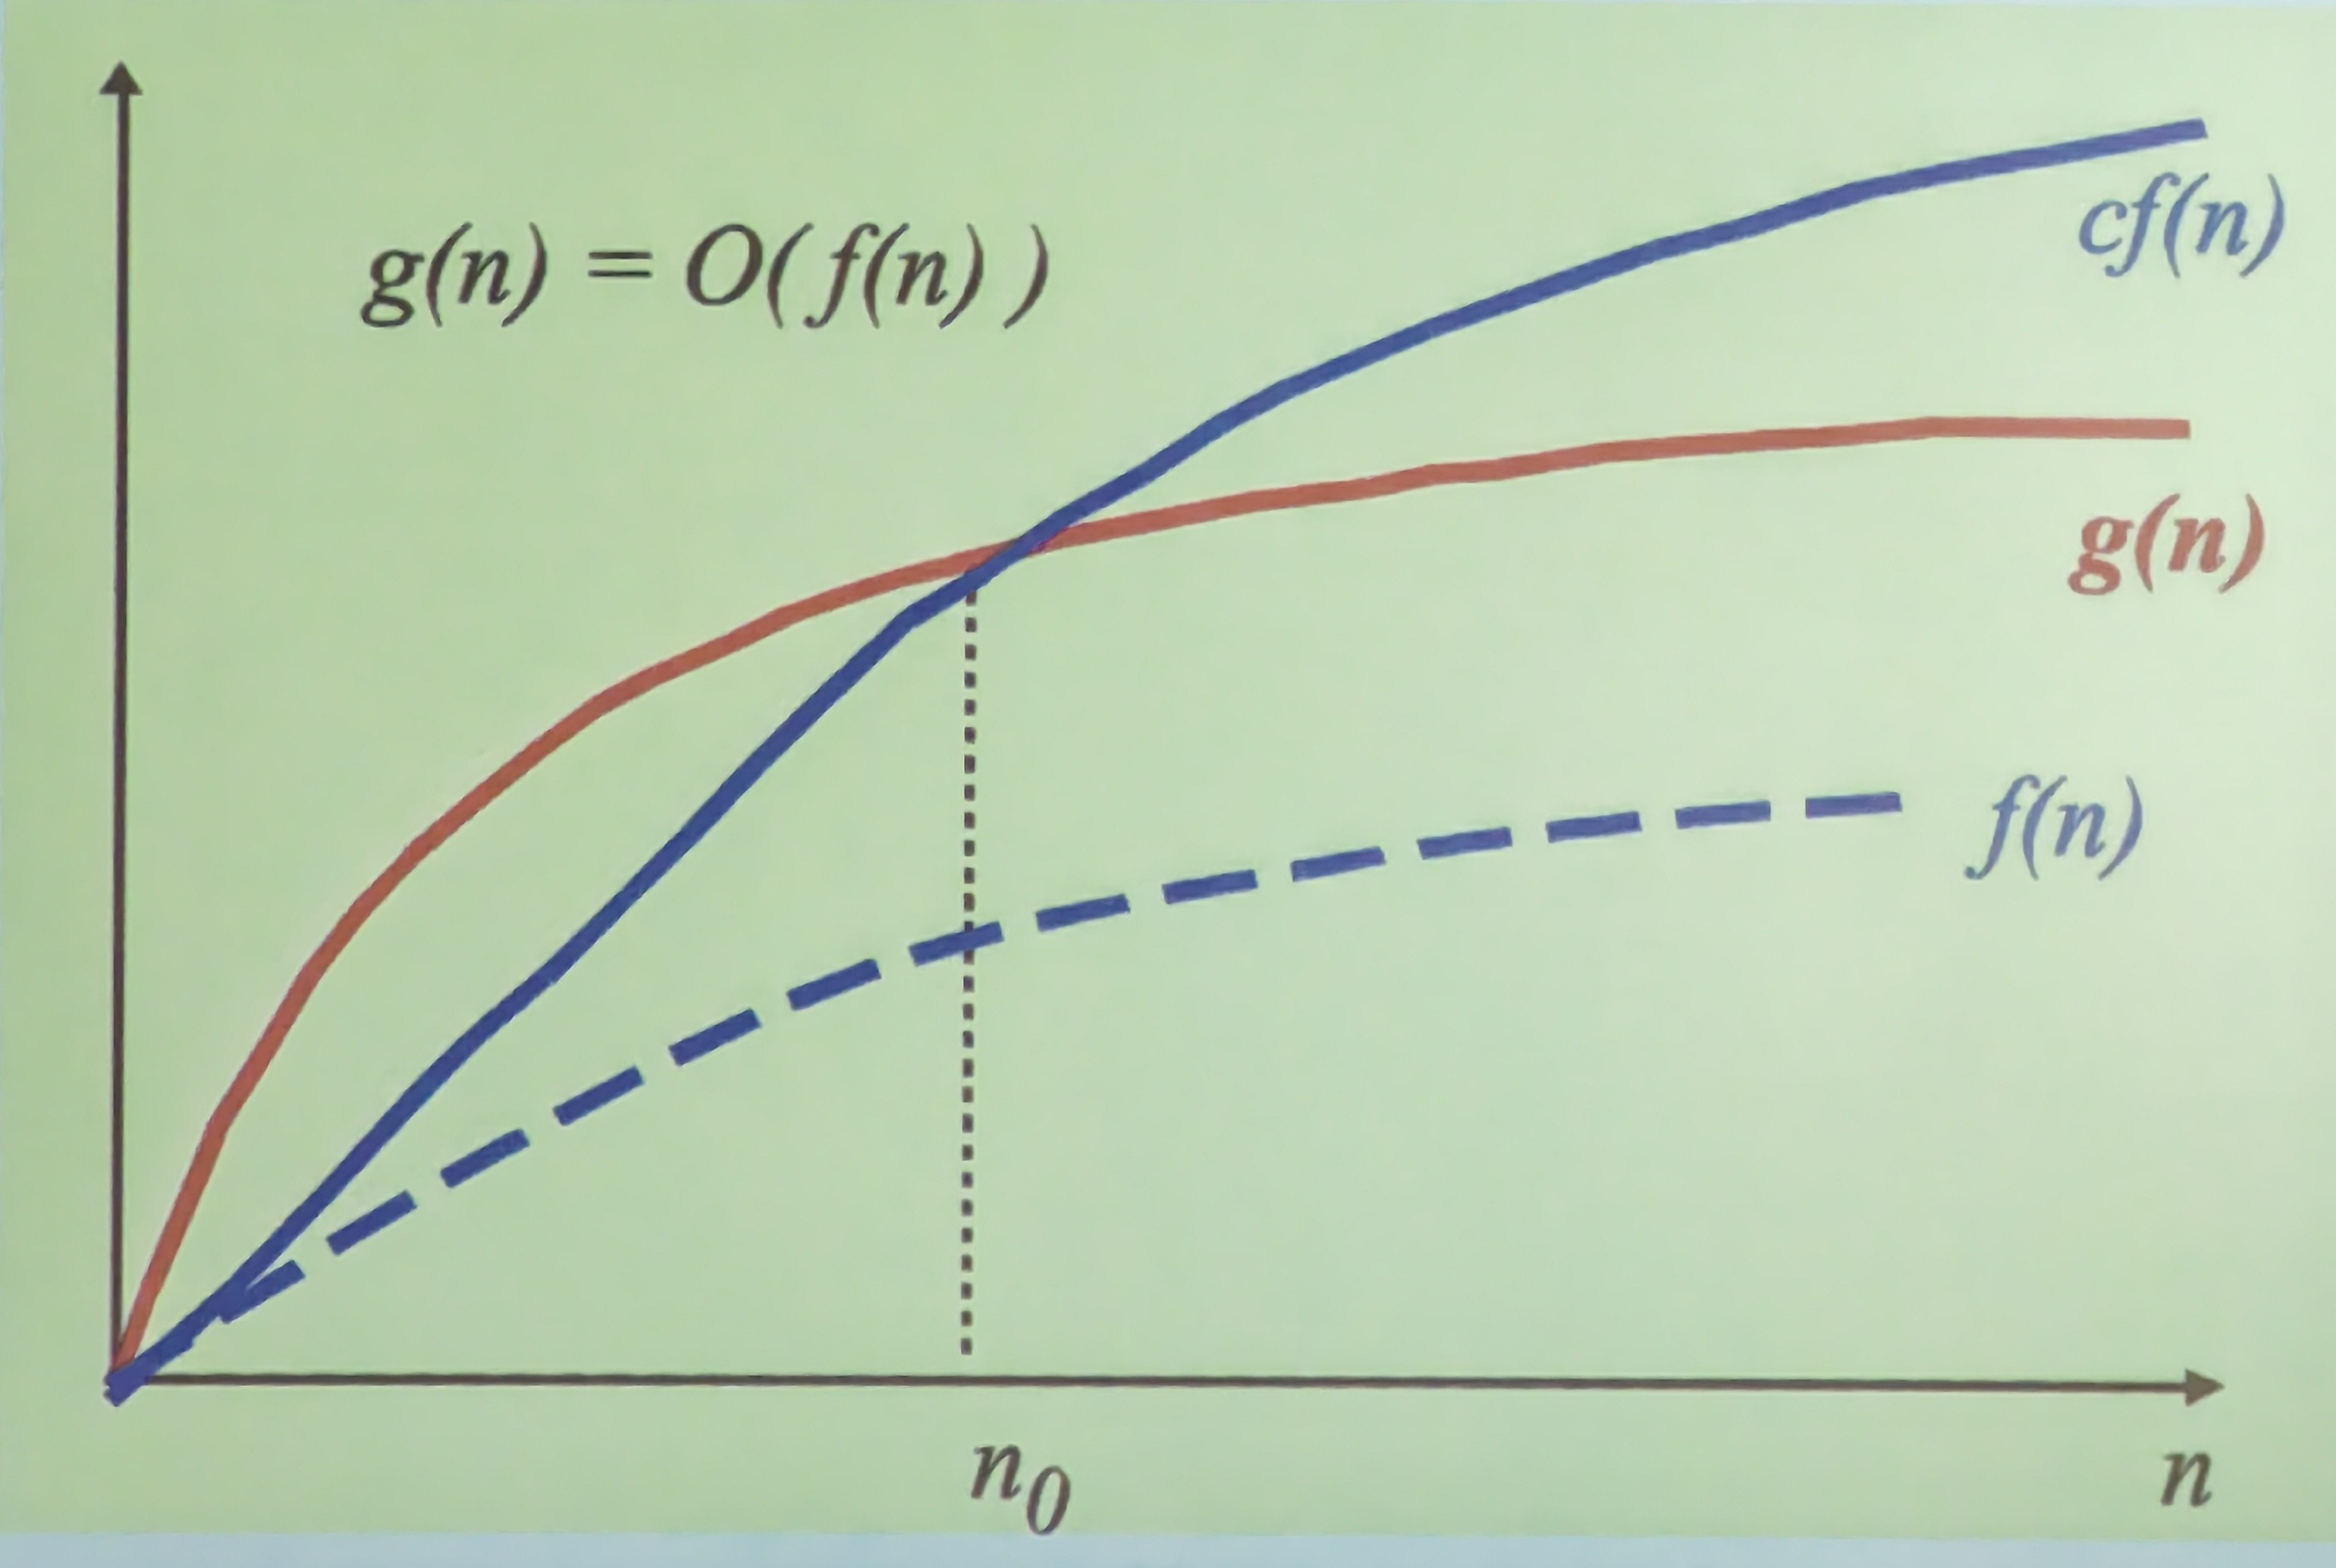
\includegraphics[width=5cm]{bigograph.jpeg}
\begin{definition}
    Una funzione \(g(n)\) appartiene all'insieme \(O(f(n))\) (si dice anche \(g(n)\) è \(O(f(n))\)) se esistono due costanti \(c > 0\) e \(n_{0} \geq 0\) tali che \(g(n) \leq cf(n)\) per ogni \(n \geq n_{0}\), ossia, da un certo punto in poi, \(g\) sta sotto una funzione "multipla" di \(f\) ("cresce al più come \(f\)").
\end{definition}
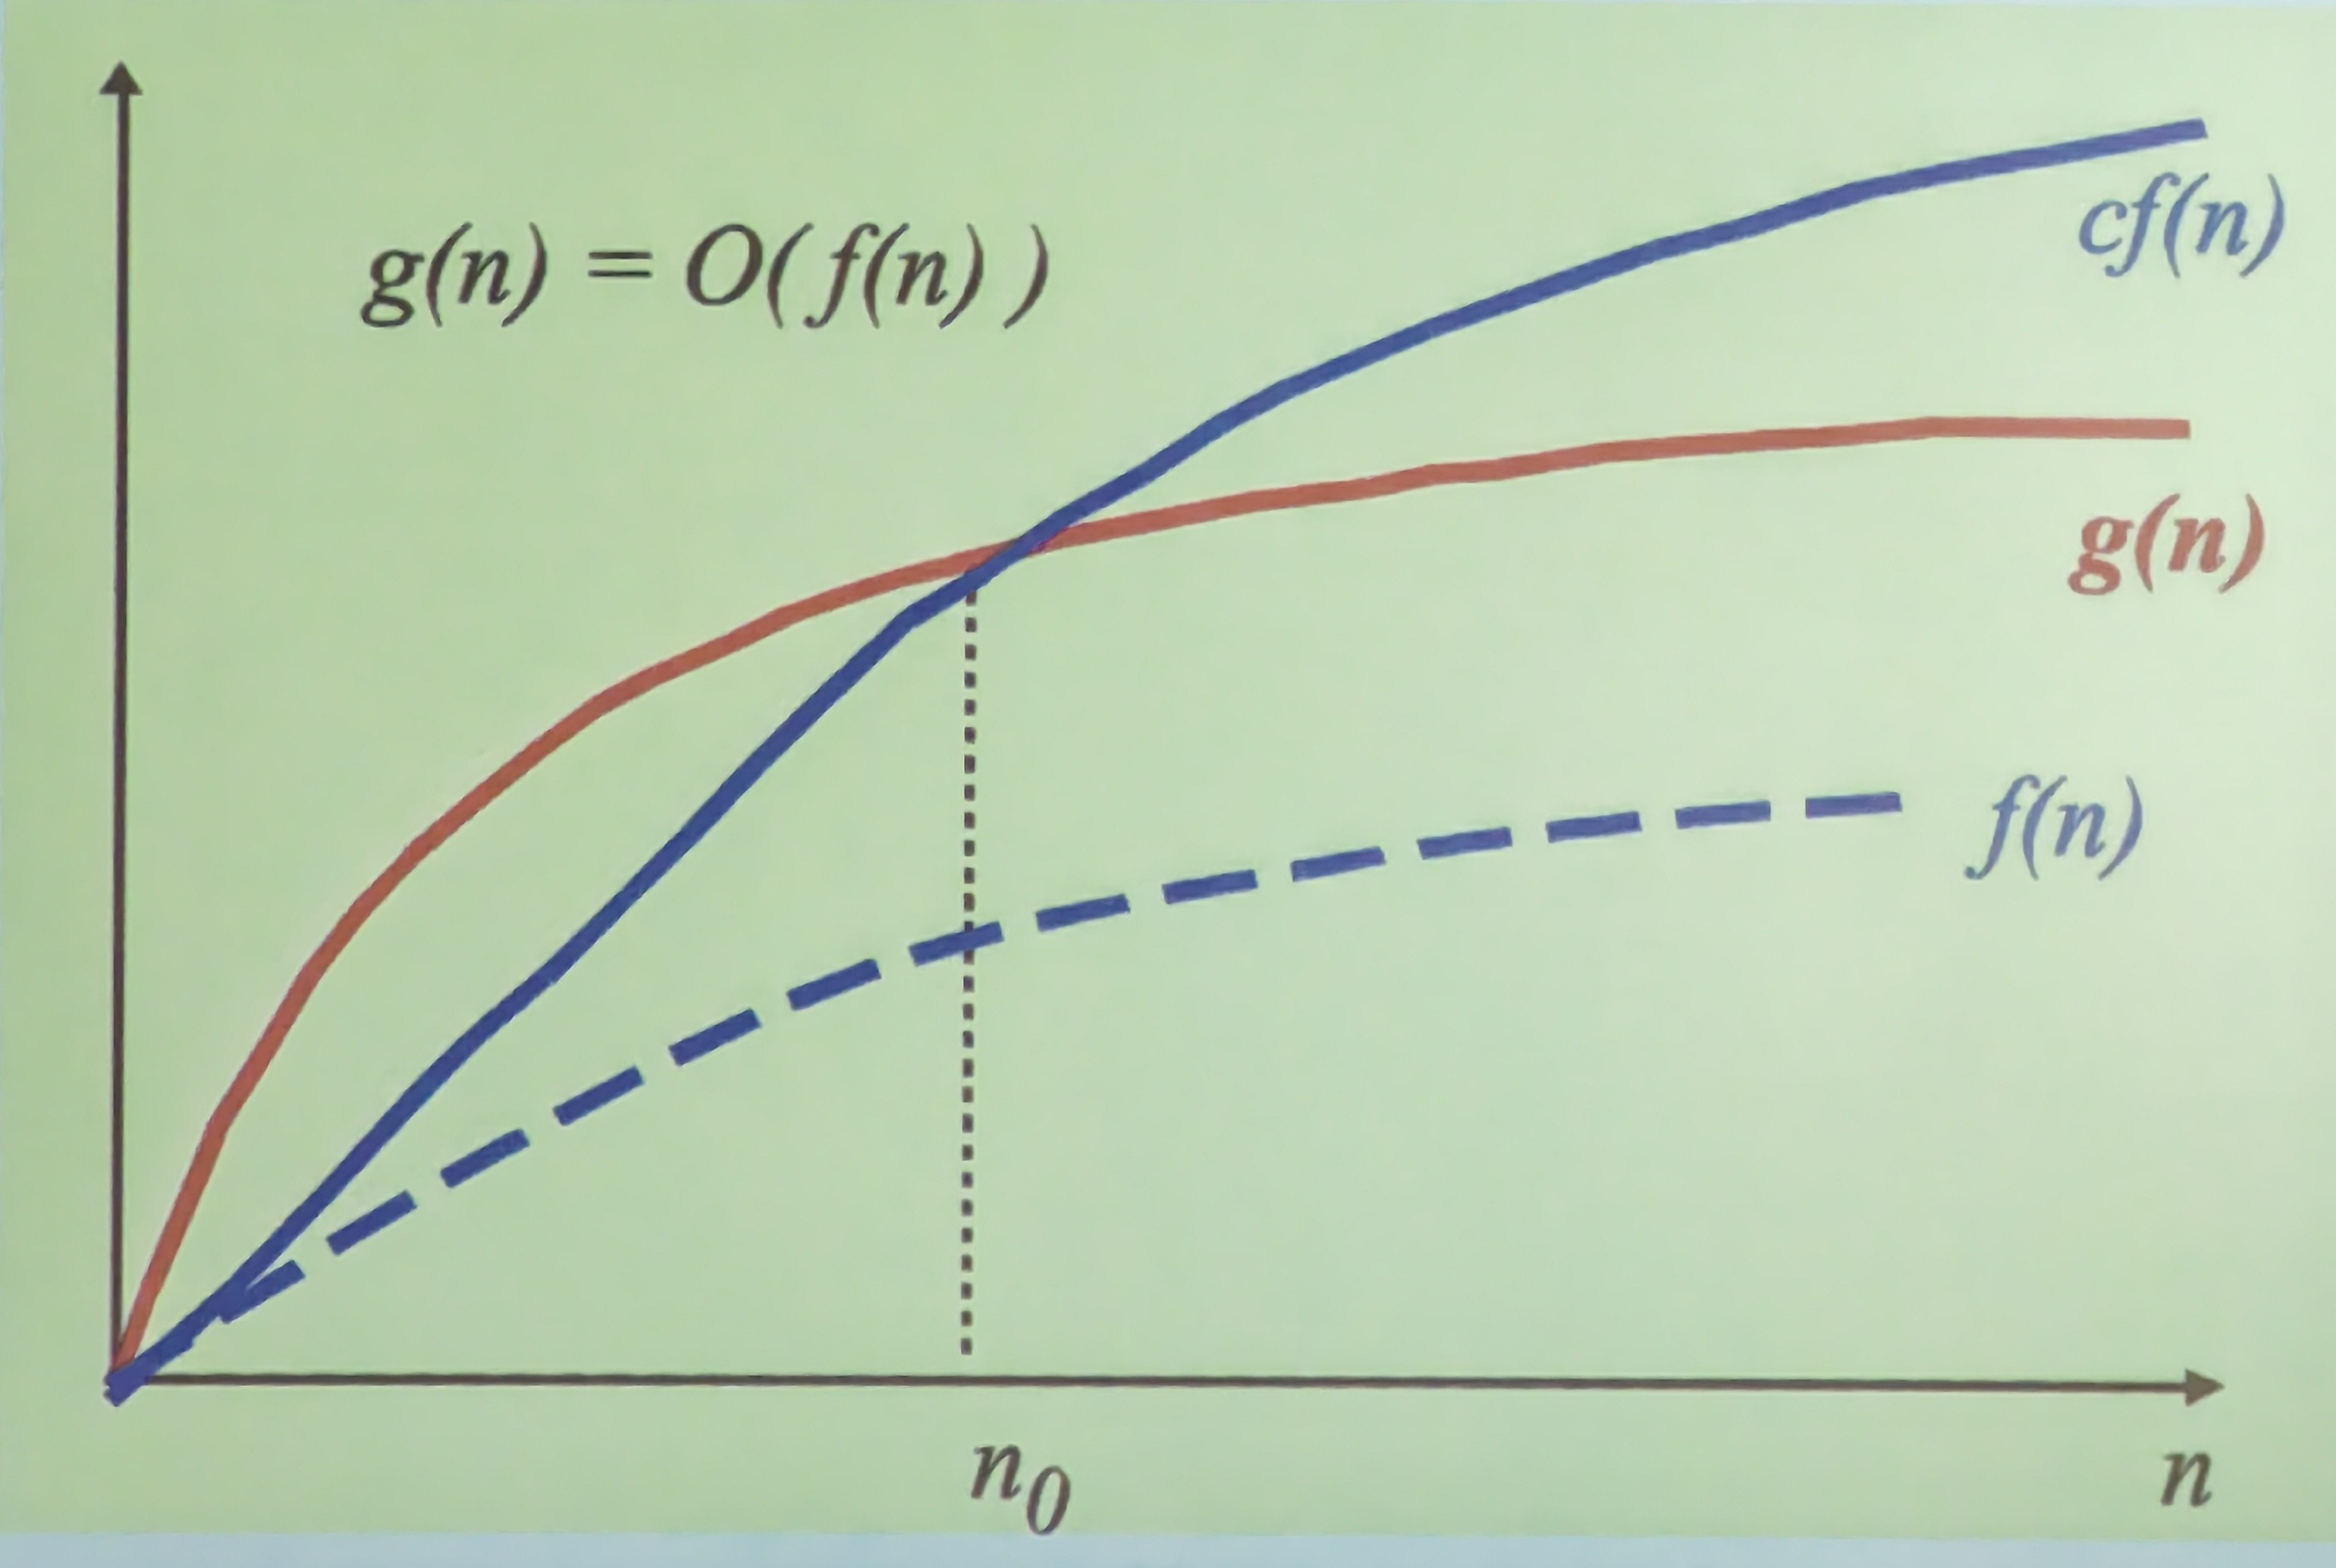
\includegraphics[width=5cm]{bigograph.jpeg}
\begin{definition}
    Una funzione \(g(n)\) appartiene all'insieme \(\Omega(f(n))\) (si dice anche \(g(n)\)) è \(\Omega(f(n))\) se esistono due costanti \(c > 0\) e \(n_{0} \geq 0\) tali che \(g(n) \geq cf(n)\) per ogni \(n \geq n_{0}\), ossia, da un certo punto in poi, \(f\) sta sopra una funzione "sottomultipla" di \(f\) ("cresce almeno come \(f\)")
\end{definition}
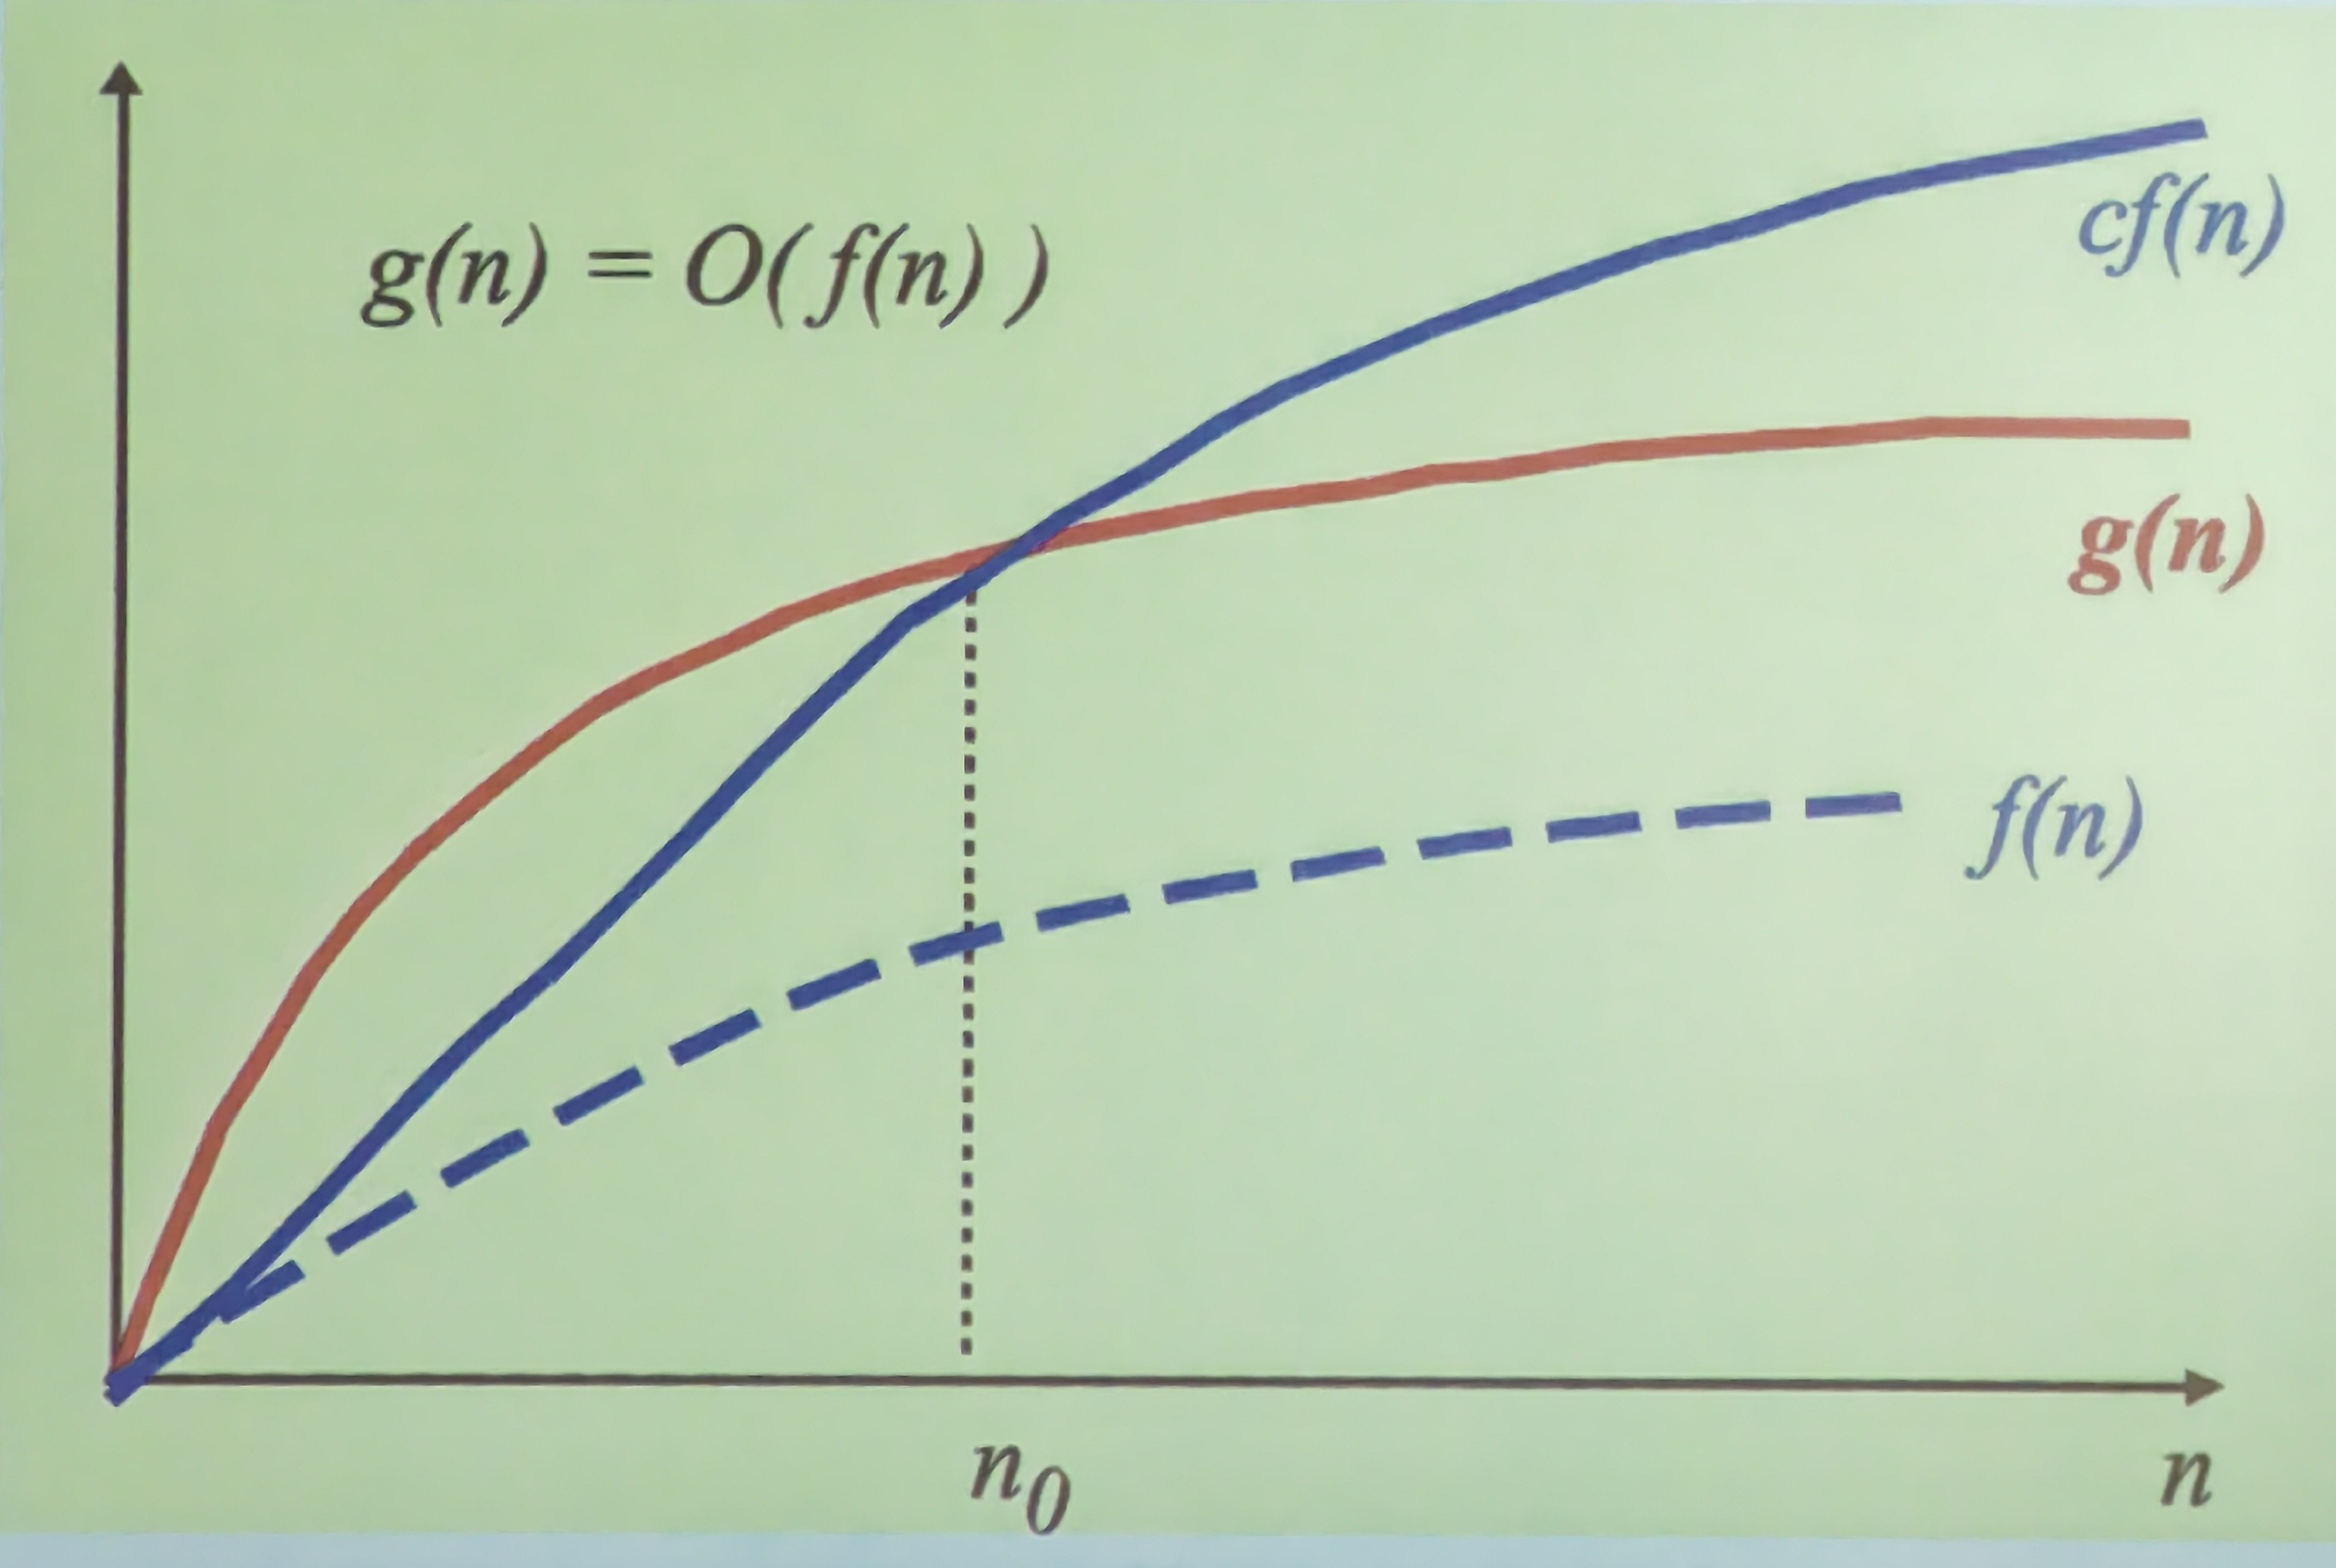
\includegraphics[width=5cm]{bigograph.jpeg}
\begin{definition}
    Una funzione \(g(n)\) appartiene all'insieme \(\Theta(f(n))\) (si dice anche \(g(n)\) è \(\Theta(f(n))\)) se esistono tre costanti \(c_{1},c_{2} > 0\) e \(n_{0} \geq 0\) tali che \(c_{1}f(n) \leq g(n) \leq c_{2}f(n)\) per ogni \(n \geq n_{0}\), ossia, da un certo punto in poi, \(f\) è compresa tra un "multiplo" di \(f\) e un "sottomultiplo" di \(f\) ("cresce come \(f\)")
\end{definition}
Per comodità si usa anche scrivere \(f(n) = O(g(n))\), e analogamente per le altre notazioni. Il simbolo \(=\) in questo caso non denota un'uguaglianza, ma l'appartenenza a un insieme.
\subsection*{Proprietà della notazione asintotica}
\subsubsection*{Transitiva}
\begin{itemize}
    \setlength\itemsep{0em}
    \item \(f(n) \text{ è } O(g(n)) \text{ e } g(n) \text{ è } O(h(n)) \text{ implica } f(n) \text{ è } O(h(n))\)
    \item \(f(n) \text{ è } \Omega(g(n)) \text{ e } g(n) \text{ è } \Omega(h(n)) \text{ implica } f(n) \text{ è } \Omega(h(n))\)
    \item \(f(n) \text{ è } \Theta(g(n)) \text{ e } g(n) \text{ è } \Theta(h(n)) \text{ implica } f(n) \text{ è } \Theta(h(n))\)
\end{itemize}
\subsubsection*{Riflessiva}
\begin{itemize}
    \setlength\itemsep{0em}
    \item \(f(n) \text{ è } O(f(n))\)
    \item \(f(n) \text{ è } \Omega(f(n))\)
    \item \(f(n) \text{ è } \Theta(f(n))\)
\end{itemize}
\subsubsection*{Simmetrica}
\(f(n) \text{ è } \Theta(g(n)) \text{ se e solo se } g(n) \text{ è } \Theta(f(n))\)
\subsubsection*{Simmetrica Trasposta}
\(f(n) \text{ è } O(g(n)) \text{ se e solo se } g(n) \text{ è } \Omega(f(n))\)
\subsubsection*{Comportamenti notevoli Intrattabili}
\begin{itemize}
    \setlength\itemsep{0em}
    \item \(\Theta(2^{n})\) esponenziale
    \item \(\Theta(n!)\) fattoriale
    \item \(\Theta(n^{n})\) esponenziale in base n
\end{itemize}
\section{Capitolo 1.2}
Formalmente, se \(i\) è un input, siano \(t(i) \text{ e } s(i)\) il tempo di esecuzione e lo spazio di memoria necessario (in aggiunta allo spazio occupato dall'input stesso) per l'esecuzione dell'algoritmo per l'input \(i\). Le seguenti funzioni risultno allora ben definite:
\begin{itemize}
    \setlength\itemsep{0em}
    \item \textbf{complessità temporale del caso peggiore}: \(T_{worst}(n) = \max\left\{t(i)|i \text{ ha dimensione }n\right\}\)
    \item \textbf{complessità temporale del caso migliore}: \(T_{best}(n) = \min\left\{t(i)|i \text{ ha dimensione }n\right\}\)
    \item \textbf{complessità temporale del caso medio}: \(T_{avg}(n) = \text{avg}\left\{t(i)|i \text{ ha dimensione }n\right\}\)
\end{itemize}
Per il caso medio, per ogni \(n\) si considerano tutti i possibili input di dimensione \(n\), siano \(i_{1},\dots, i_{N}\), e si fa la media aritmetica dei tempi:
\begin{equation}
    T_{avg}(n) = \frac{t(i_{1})+\dots+t(i_{N})}{N}
\end{equation}
Usiamo la media pesata se i possibili input non sono equiprobabili.
\\Vi sono quindi nove possibili affermazioni sulla complessità di un algoritmo, non tutte però indipendenti tra loro nè ugualmente interessanti. In particolare, si ha che se \(T_{worst}(n)=O(f(n))\), allora anche \(T_{avg}(n)=O(f(n))\) e \(T_{best}(n)=O(f(n))\), e simmetricamente se \(T_{best}(n)=\Omega(f(n))\), allora anche \(T_{avg}(n)=\Omega(f(n))\) e \(T_{worst}(n)=\Omega(f(n))\).
\begin{itemize}
    \setlength\itemsep{0em}
    \item un algoritmo ha complessità \(O(f(n)) \text{ se } T_{worst}(n)=O(f(n))\). Ossia \(f(n)\) è una delimitazione superiore del tempo di calcolo: al crescere di \(n\) il tempo di calcolo non cresce più di \(f(n)\), qualunque sia l'input.
    \item un algoritmo ha complessità \(\Omega(f(n)) \text{ se } T_{best}(n)=\Omega(f(n))\). Ossia \(f(n)\) è una delimitazione inferiore del tempo di calcolo: al crescere di \(n\) il tempo di calcolo cresce almeno come \(f(n)\), qualunque sia l'input.
    \item un algoritmo ha complessità \(\Theta(f(n)) \text{ se ha complessità } O(f(n)) \text{ e } \Omega(f(n))\). Ossia, \(f(n)\) è una delimitazione sia inferiore che superiore del tempo di calcolo, qualunque sia l'input.
\end{itemize}
Il caso migliore è di solito scarsamente interessante, poichè riguarda input molto particolari. Il caso medio è significativo solo se la distribuzione delle probabilità riflette la situazione reale di uso dell'algoritmo. Il caso peggiore è la complessità che si studia di solito, poiché è l'unica che fornisce la garanzia che in ogni caso il tempo di esecuzione non sarà maggiore di un certo tempo prevedibile.\\
Nel caso di un algoritmo randomizzato, possiamo calcolare la media (pesata) dei possibili tempi di computazione per \textit{uno stesso input (expected running time)}:
\begin{equation}
    T_{exp}(i) = \mathbb{E}\left[t(i,c)\right]
\end{equation}
\textit{worst case expected running time}:
\begin{equation}
    T_{exp\_worst}(n) = \max\left\{T_{exp}(i)|i \text{ ha dimensione }n\right\}
\end{equation}
Nel confronto precedente abbiamo assunto che l'algoritmo randomizzato fornisca sempre il risultato corretto (algoritmi Las Vegas). Alcuni tipi di algoritmi randomizzati (Monte Carlo) possono anche fornire un risultato errato (forniscono comunque il risultato giusto con probabilità \(> 0\)). In questo caso la ripetizione dell'esecuzione permette di limitare la probabilità di sbagliare. Il vantaggio si ha tipicamente in casi in cui l'algoritmo deterministico è molto inefficiente.
\subsection*{Complessità dei problemi}
\begin{itemize}
    \setlength\itemsep{0em}
    \item \textbf{delimitazione superiore} \textit{Un problema ha complessità} \(O(f(n))\) se esiste un algoritmo di complessità \(O(f(n))\) che lo risolve. Ossia, è possibile risolvere il problema in un tempo che cresca non più di \(f(n)\).
    \item \textbf{delimitazione inferiore} \textit{Un problema ha complessità} \(\Omega(f(n))\) se tutti i possibili algoritmi risolventi hanno complessità \(\Omega(f(n))\). Ossia, non è possibile risolvere il problema in un tempo che cresca meno di \(f(n)\).
\end{itemize}
Quindi, per trovare una delimitazione superiore \(f(n)\) alla complessità del problema, è sufficiente (e necessario) trovare \textit{un} algoritmo che risolva il problema in un tempo \(O(f(n))\), mentre, per trovare una delimitazione inferiore \(g(n)\), è necessario dimostrare che \textit{qualunque} possibile algoritmo deve impiegare un tempo \(\Omega(g(n))\). Non basta quindi che tutti gli algoritmi conosciuti abbiano complessità \(\Omega(g(n))\).\\
Un problema algoritmico, può essere \textit{aperto (o con gap algoritmico)} o \textit{chiuso}. Un problema aperto può venire chiuso, ma non viceversa. Un problema è chiuso se si conoscono limite superiore e inferiore coincidenti, ossia:
\begin{itemize}
    \setlength\itemsep{0em}
    \item esiste un algoritmo risolvente di complessità \(O(f(n))\)
    \item si è dimostrato che qualunque algoritmo risolvente deve avere complessità \(\Omega(f(n))\), ossia non può esistere un algoritmo di complessità inferiore a \(\Omega(f(n))\).
\end{itemize}
Si è quindi dimostrato che l'algoritmo risolvente è \textbf{ottimo}. Saranno possibili solo miglioramenti marginali, per esempio per una costante additiva o moltiplicativa.\\
Un problema è aperto se (tutte le) delimitazioni inferiori e superiori differiscono, ossia:
\begin{itemize}
    \setlength\itemsep{0em}
    \item il miglior algoritmo risolvente noto ha complessità \(O(f(n))\)
\end{itemize}
Un gap algoritmico può essere chiuso in due modi:
\begin{itemize}
    \setlength\itemsep{0em}
    \item dal di sopra: si trova un algoritmo migliore, abbassando così il limite superiore; se si trova un algoritmo di complessità coincidente con il limite inferiore, tale algoritmo è ottimo e il problema è chiuso.
    \item dal di sotto: si riesce a dimostrare un limite inferiore più alto; se questo coincide con la complessità dell'algoritmo migliore esistente, si è dimostrato che l'algoritmo è ottimo e il problema è chiuso.
\end{itemize}
\textbf{Non tutti i problemi sono risolubili}
\end{document}